\documentclass{Resources/cquicc}
\subjectarea{Report}
\keywords{component, formatting, style, styling, insert.}

\begin{document}
\firstpage{1}
\title{Title}
\author{John Doe}
\date{\today}
\maketitle
\setcounter{tocdepth}{2}
\begin{abstract}
This document is a model and instructions for \LaTeX.
*ADVISABLE: Do Not Use Symbols, Special Characters, Footnotes, 
or Math in Paper Title or Abstract.
\end{abstract}
\section{Introduction}
\lipsum[1]
\begin{figure}[h]
    \centering
    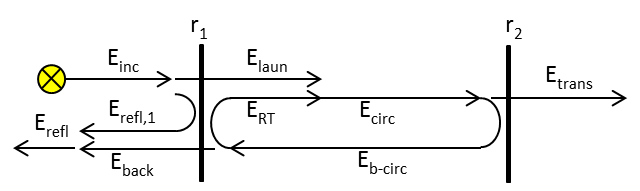
\includegraphics[width=\linewidth]{images/Schematic_of_the_Fabry-Perot_interferometer.png}
    \caption{Schematic of Fabry Perot Interferometer. We have considered two mirrors $M1$ and $M2$ with field reflectivities $r_1$ and $r_2$ respectively. }
    \label{fig:schematic_fp_cavity}
\end{figure}
\subsection{Resonant properties}
We assume that the source is emitting a single-frequency light incident on the cavity from the left. There are two mirrors \textit{$M_1$}, \textit{$M_2$} with reflectivities \textit{$r_1$}, and \textit{$r_2$}. 
\subsubsection{Circulating Field : }$\vec{E}_{\text{\text{circ}}}$, inside the cavity is a vector sum of the fraction of the incident field, $\vec{E}_{\text{}inc}$, and the contribution of the circulating signal from the previous cycle $\vec{E}_{\text{\text{circ}}}$, which is again bouncing off the \textit{$M_1$}. The total circulating field just inside the mirror \textit{$M_1$} can thus be written as:
\begin{equation}
    \vec{E}_{\text{circ}} = j t_1 \vec{E}_{\text{inc}} + g_{\text{rt}}(\omega) \vec{E}_{\text{circ}}
    \label{equation_circulating}
\end{equation}
where, $g_{\text{rt}}$  is the net complex round trip gain. Although, this is a passive cavity, the choice of words \textit{complex round trip gain}, comes from the reference which extends the same analysis to lasers. In our case, $|g_{\text{rt}}(\omega)|<1$. We have assumed a lossless cavity.
\subsubsection{Complex Round Trip Gain} The round trip length of the cavity is assumed to be 2L. The incident wave has a frequency $\omega$ and propagation constant $k = \omega/c$. Hence, the phase shift associated with a round trip is $\exp(-j2\omega L/c)$. \par 
The circulating field will return to the reference point inside the mirror $M_1$ after one round trip with the complex round trip gain given by, 
\begin{equation}
    g_{\text{rt}}(\omega) = r_1r_2\times \exp(j2\omega L/c)
\end{equation}
\par
Although we have assumed a lossless cavity, it can be easily included in the amplitude as multiplication by the factor $\exp (-\alpha_0 l) $ in the complex round trip gain, where $\alpha_0$ is the absorption coefficient.  \par
\subsubsection{Cavity Resonance}
Eq. \ref{equation_circulating}, can be re-written as,
\begin{equation}
\begin{split}
    \vec{E}_{\text{circ}} & = j \sqrt{(1-r_1^2)} \vec{E}_{\text{inc}} + g_{\text{rt}}(\omega) \vec{E}_{\text{circ}} \\
    & = j \sqrt{(1-r_1^2)} \vec{E}_{\text{\text{inc}}} + r_1r_2\times \exp(j2\omega L/c)  \vec{E}_{\text{circ}}\\
    \frac{\vec{E}_{\text{circ}}}{\vec{E}_{\text{inc}}} & = \frac{j\sqrt{(1-r_1^2)}}{1-r_1r_2\times \exp(j2\omega L/c)}
\end{split}
\label{eqn:cavity_resonance}
\end{equation}
\begin{figure}
    \centering
    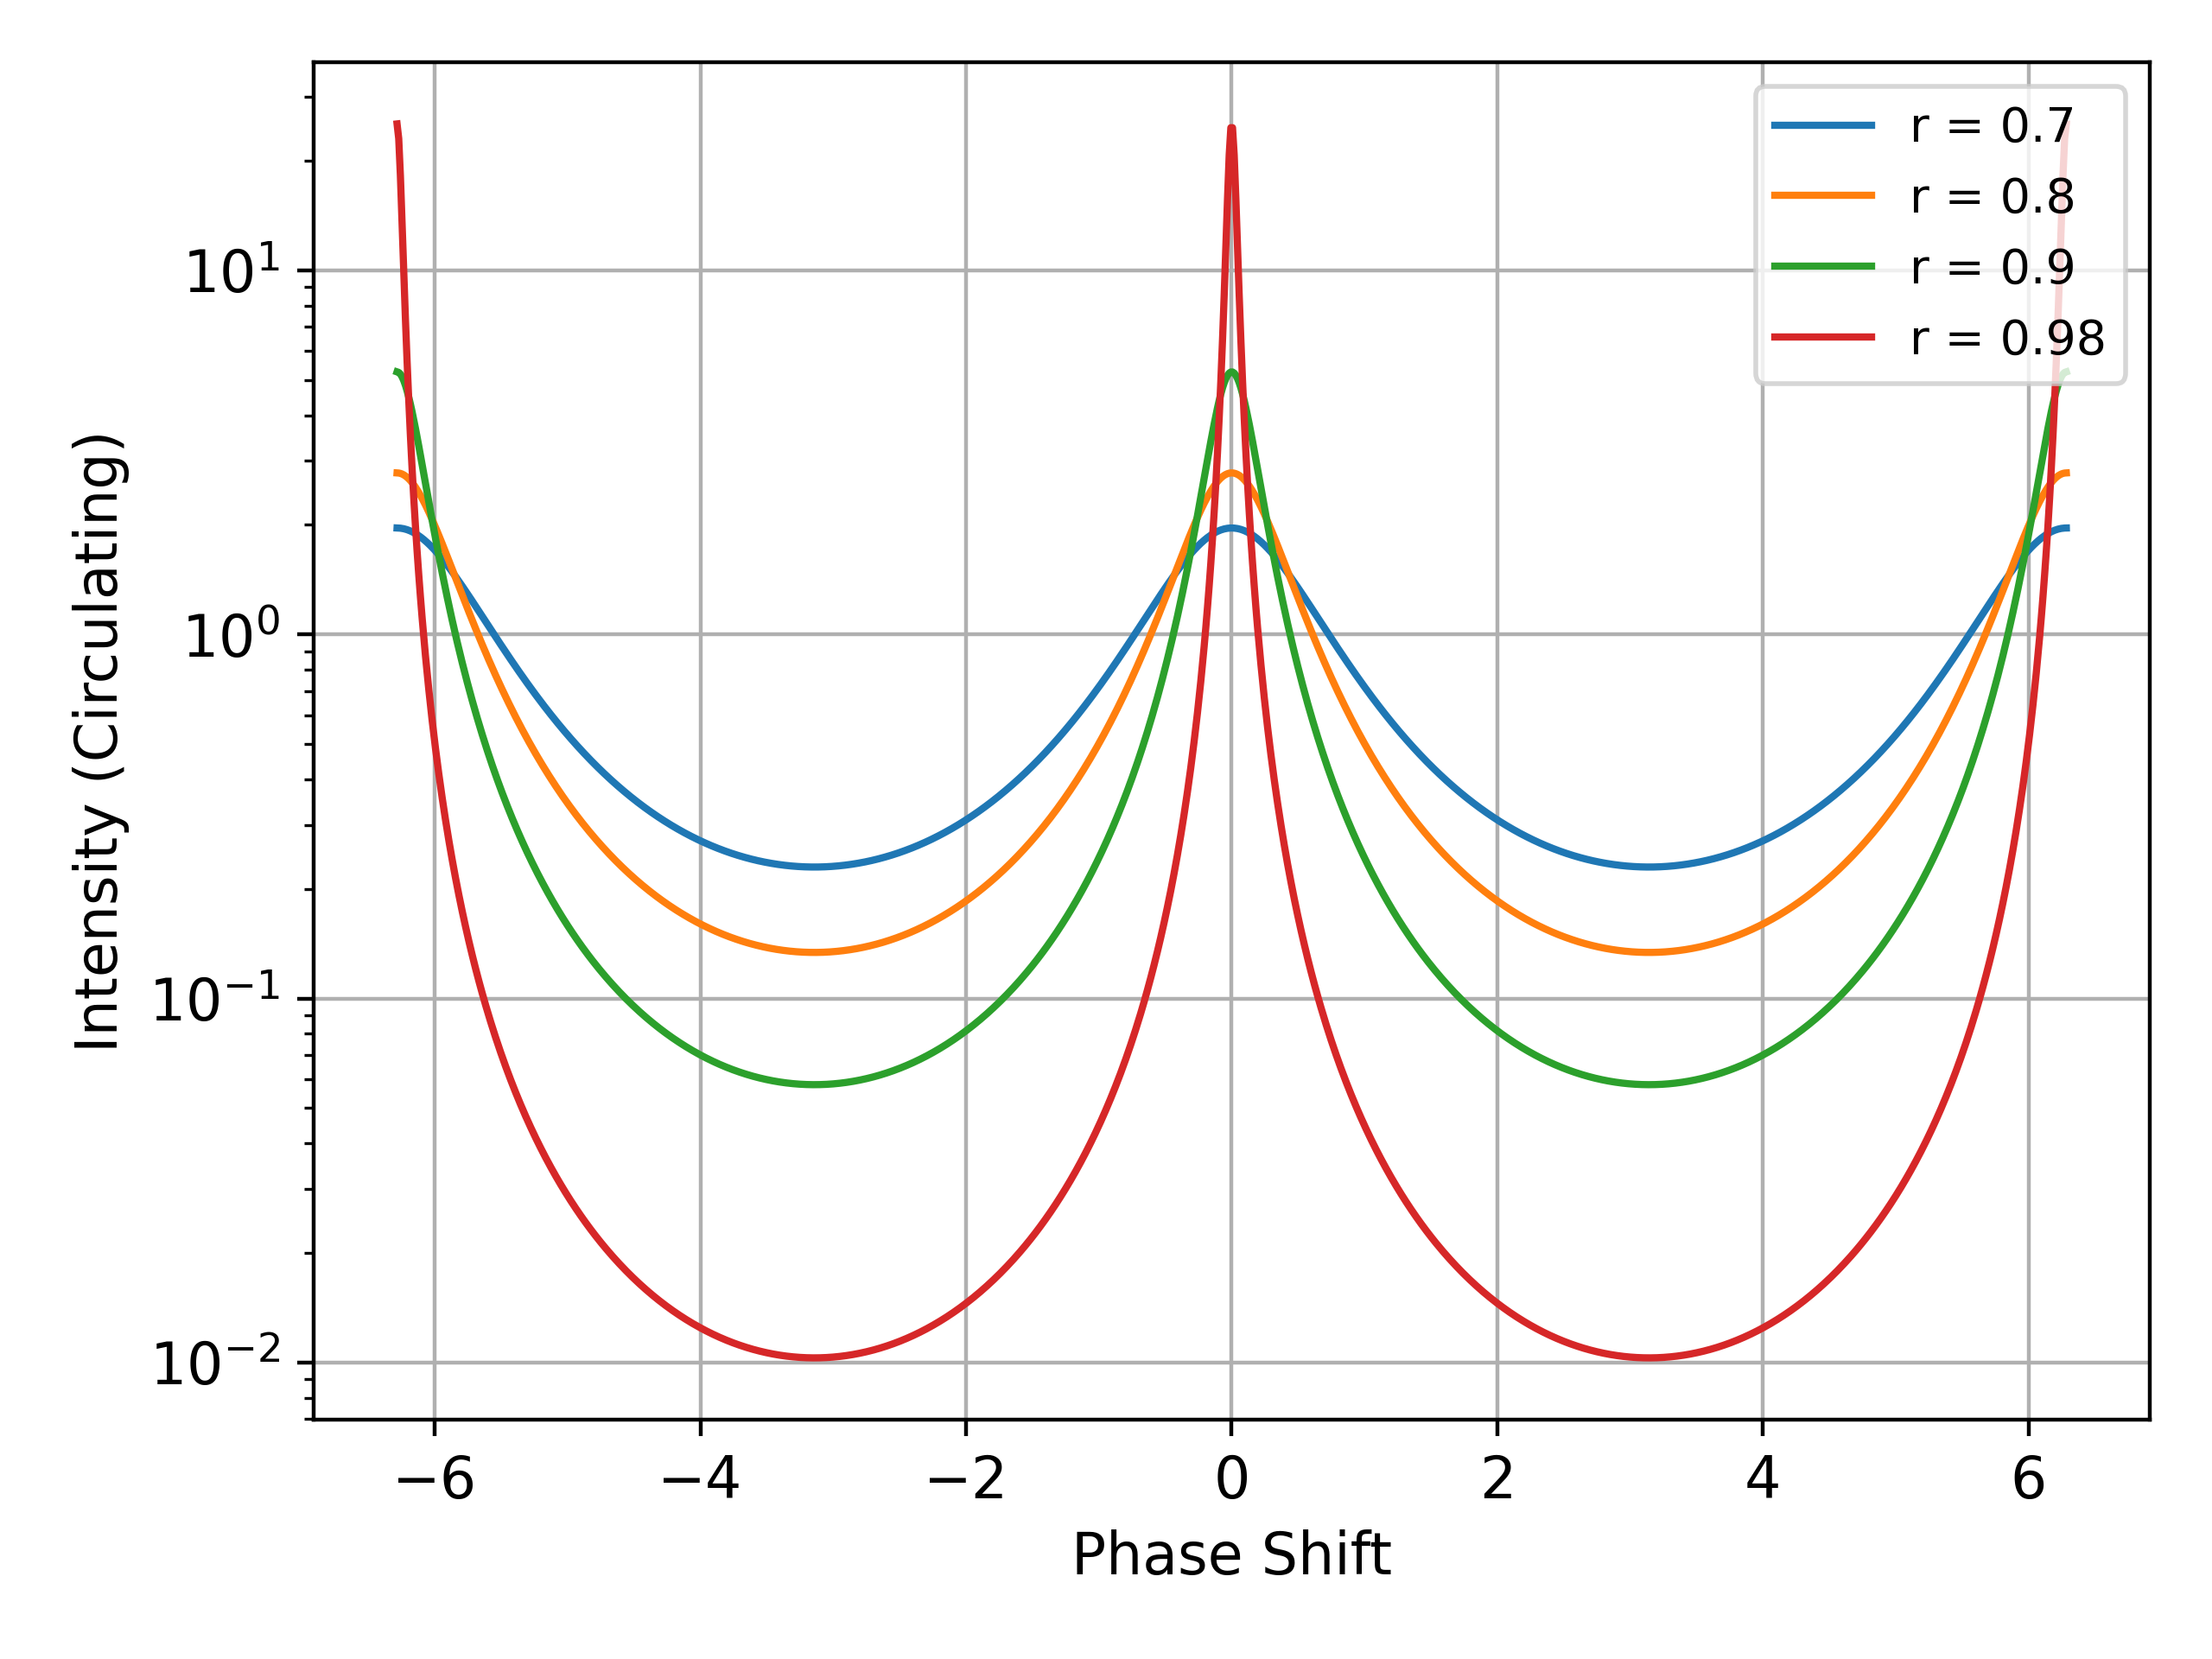
\includegraphics[width=\linewidth]{images/Cavity_resonance.png}
    \caption{Circulating Intensity within the cavity at different $r$.}
    \label{fig:cavity_resonance}
\end{figure}
Plotting the intensity ${I_{\text{circ}}}/{I_{\text{inc}}} = |{\vec{E}_{\text{circ}}}/{\vec{E}_{\text{inc}}}|^2$ in Fig. \ref{fig:cavity_resonance}, we can see that the system exhibits resonance when $2\omega L /c = 2 \pi$
\subsubsection{Circulating Intensity Magnification} 
The magnification of circulating intensity can be found easily from expression in Eq. \ref{eqn:cavity_resonance}. Let us assume $r_1 = r_2 = r$, and assuming negligible losses, we get the electric field at resonance $\omega_{res} = n\pi c/L$,
\begin{equation}
    \begin{split}
            \frac{\vec{E}_{\text{circ}}}{\vec{E}_{\text{inc}}}\Bigg|_{\omega = \omega_{res}} & = \frac{j\sqrt{(1-r^2)}}{1-r^2} = \frac{j}{\sqrt{(1-r^2)}} 
    \end{split}
\end{equation}
Hence, we can say that the circulating intensity magnification for a symmetric cavity is given by, 
\begin{equation}
\label{eqn: circulating_intensity_max}
    \frac{I_{\text{circ}}}{I_{\text{inc}}} \approx \Bigg| \frac{1}{1-r^2} \Bigg | = \Bigg| \frac{1}{T} \Bigg |  
\end{equation}
\subsubsection{Transmitted Cavity Field}
The transmitted electric field from the mirror $M2$ in Fig. \ref{fig:schematic_fp_cavity} will be a fraction of the light circulating in the cavity given by, 
\begin{equation}
    \begin{split}
        \vec{E}_{\text{trans}} = jt_2 \times \exp(j\omega L / c) \times \vec{E}_{\text{circ}}
    \end{split}
\end{equation}
Here, only the one-sided length of the cavity is considered, instead of the round trip length in the previous case. Hence, the total transmission through the cavity can be written as, 
\begin{equation}
    \begin{split}
        \vec{E}_{\text{trans}} & = \frac{j^2t_1t_2 \times \exp(j\omega L / c) }{1-r_1r_2\times \exp(j2\omega L/c)} \times{\vec{E}_{\text{inc}}} \\
        \Bigg | \frac{\vec{E}_{\text{trans}}}{{\vec{E}_{\text{inc}}}} \Bigg| & = \frac{-t_1t_2 \times \exp(j\omega L / c) }{1-r_1r_2\times \exp(j2\omega L/c)} \\
        & = \frac{-t_1t_2 \times \exp(j\omega L / c) }{1-g_{\text{rt}}(\omega)}
    \end{split}
\end{equation}

\subsubsection{Reflected Cavity Fields}
Before delving into mathematics, let us analyse the reflected field from the cavity using the same approach as followed in the transmitted cavity field subsection. Assuming a symmetric mirror case with R = 99\%, and input power of 1~mW, circulating power from Eq. \ref{eqn: circulating_intensity_max} would be 100~mW. Since, the output mirror has a power transmission of 1\%, the input mirror of the same make, should output 1~mW of power. It would seem that for 1~mW of input power, we are getting 2~mW of cumulative power from the input and output mirrors. \par
The conundrum can be resolved easily if we understand that the reflected electric field $\vec{E}_{\text{refl}}$ is a sum of \textit{promptly reflected beam} from the mirror $M1$ and the \textit{leakage beam} from within the cavity. The \textit{leakage beam} represents the component of circulating field $\vec{E}_{\text{circ}}$ that was transmitted from the mirror $M1$. It had left the same point one round trip earlier and travelled around the cavity. Instead of being reflected by $M1$, it was transmitted through. The value of this component is given by $jt_1(g_{\text{rt}}/r1)\times \vec{E}_{\text{circ}}$. The round trip gain has been divided by $r_1$ because the wave doesn't bounce off the mirror $M1$. The total reflected wave is given by, 
\begin{equation}
    \label{eqn: reflected_wave}
    \begin{split}
    \vec{E}_{\text{refl}} & = r_1 \vec{E}_{\text{inc}} + jt_1(g_{\text{rt}}(\omega)/r_1)\times \vec{E}_{\text{circ}} \\
    \frac{\vec{E}_{\text{refl}}}{\vec{E}_{\text{inc}}} & = r_1 - \frac{t_1^2}{r_1}\frac{g_{\text{rt}}(\omega)}{1-g_{\text{rt}}(\omega)}
    \end{split}
\end{equation}
The form of Eq. \ref{eqn: reflected_wave} shows that the reflected light from the cavity is made up of \textit{promptly reflected beam} and a part of transmitted component \textit{leakage beam} from within the cavity. Let me rearrange the terms of Eq. \ref{eqn: reflected_wave} to define \textit{reflection coefficient} $F(\omega)$ written in terms of free spectral range (FSR) of the cavity. $\Delta \nu_{FSR} = c/2nL$, where $n$ is the refractive index. For a passive cavity in air, it is unity. 
\begin{equation}
    \label{eqn: reflection coefficient}
    F(\omega) = \dfrac{\vec{E}_{\text{refl}}}{\vec{E}_{\text{inc}}}  = \dfrac{r_1 - r_2 \exp\Big(\dfrac{j\omega}{\Delta \nu_{FSR}}\Big)}{1-r_1r_2\exp\Big(\dfrac{j\omega}{\Delta \nu_{FSR}}\Big)}
\end{equation}
If we assume a symmetric cavity, from Eq. \ref{eqn: reflection coefficient}, we can see that $F(\omega) = 0$ on resonance. The plot in Fig. \ref{fig:reflection_coefficient} shows the intensity and phase of the reflected light. 
\subsubsection{Cavity Stabilisation}
We can see that the reflected intensity is symmetric about resonance. It is easy to see that the transmitted light would show a complementary and symmetric resonant behaviour around resonance. The transmitted intensity would be maximum at resonance and will fall off on either side. The problem with using transmitted intensity as an error signal is our inability to differentiate between different sources of fluctuations. For example, a change in frequency would lead to a decrease in the intensity of transmitted light, but so would a change in intensity itself. Hence, we should look at the reflected light given by Eq. \ref{eqn: reflection coefficient}. Although the intensity is symmetric about resonance, the phase is asymmetric and can be used to determine which side of resonance we are on. The PDH locking technique discussed in the next section uses the reflected light and tries to keep it at minimum, effectively decoupling frequency and intensity noise. Measuring the phase of the reflected light will allow us to know which side of resonance we are on. 
\begin{figure}
    \centering
    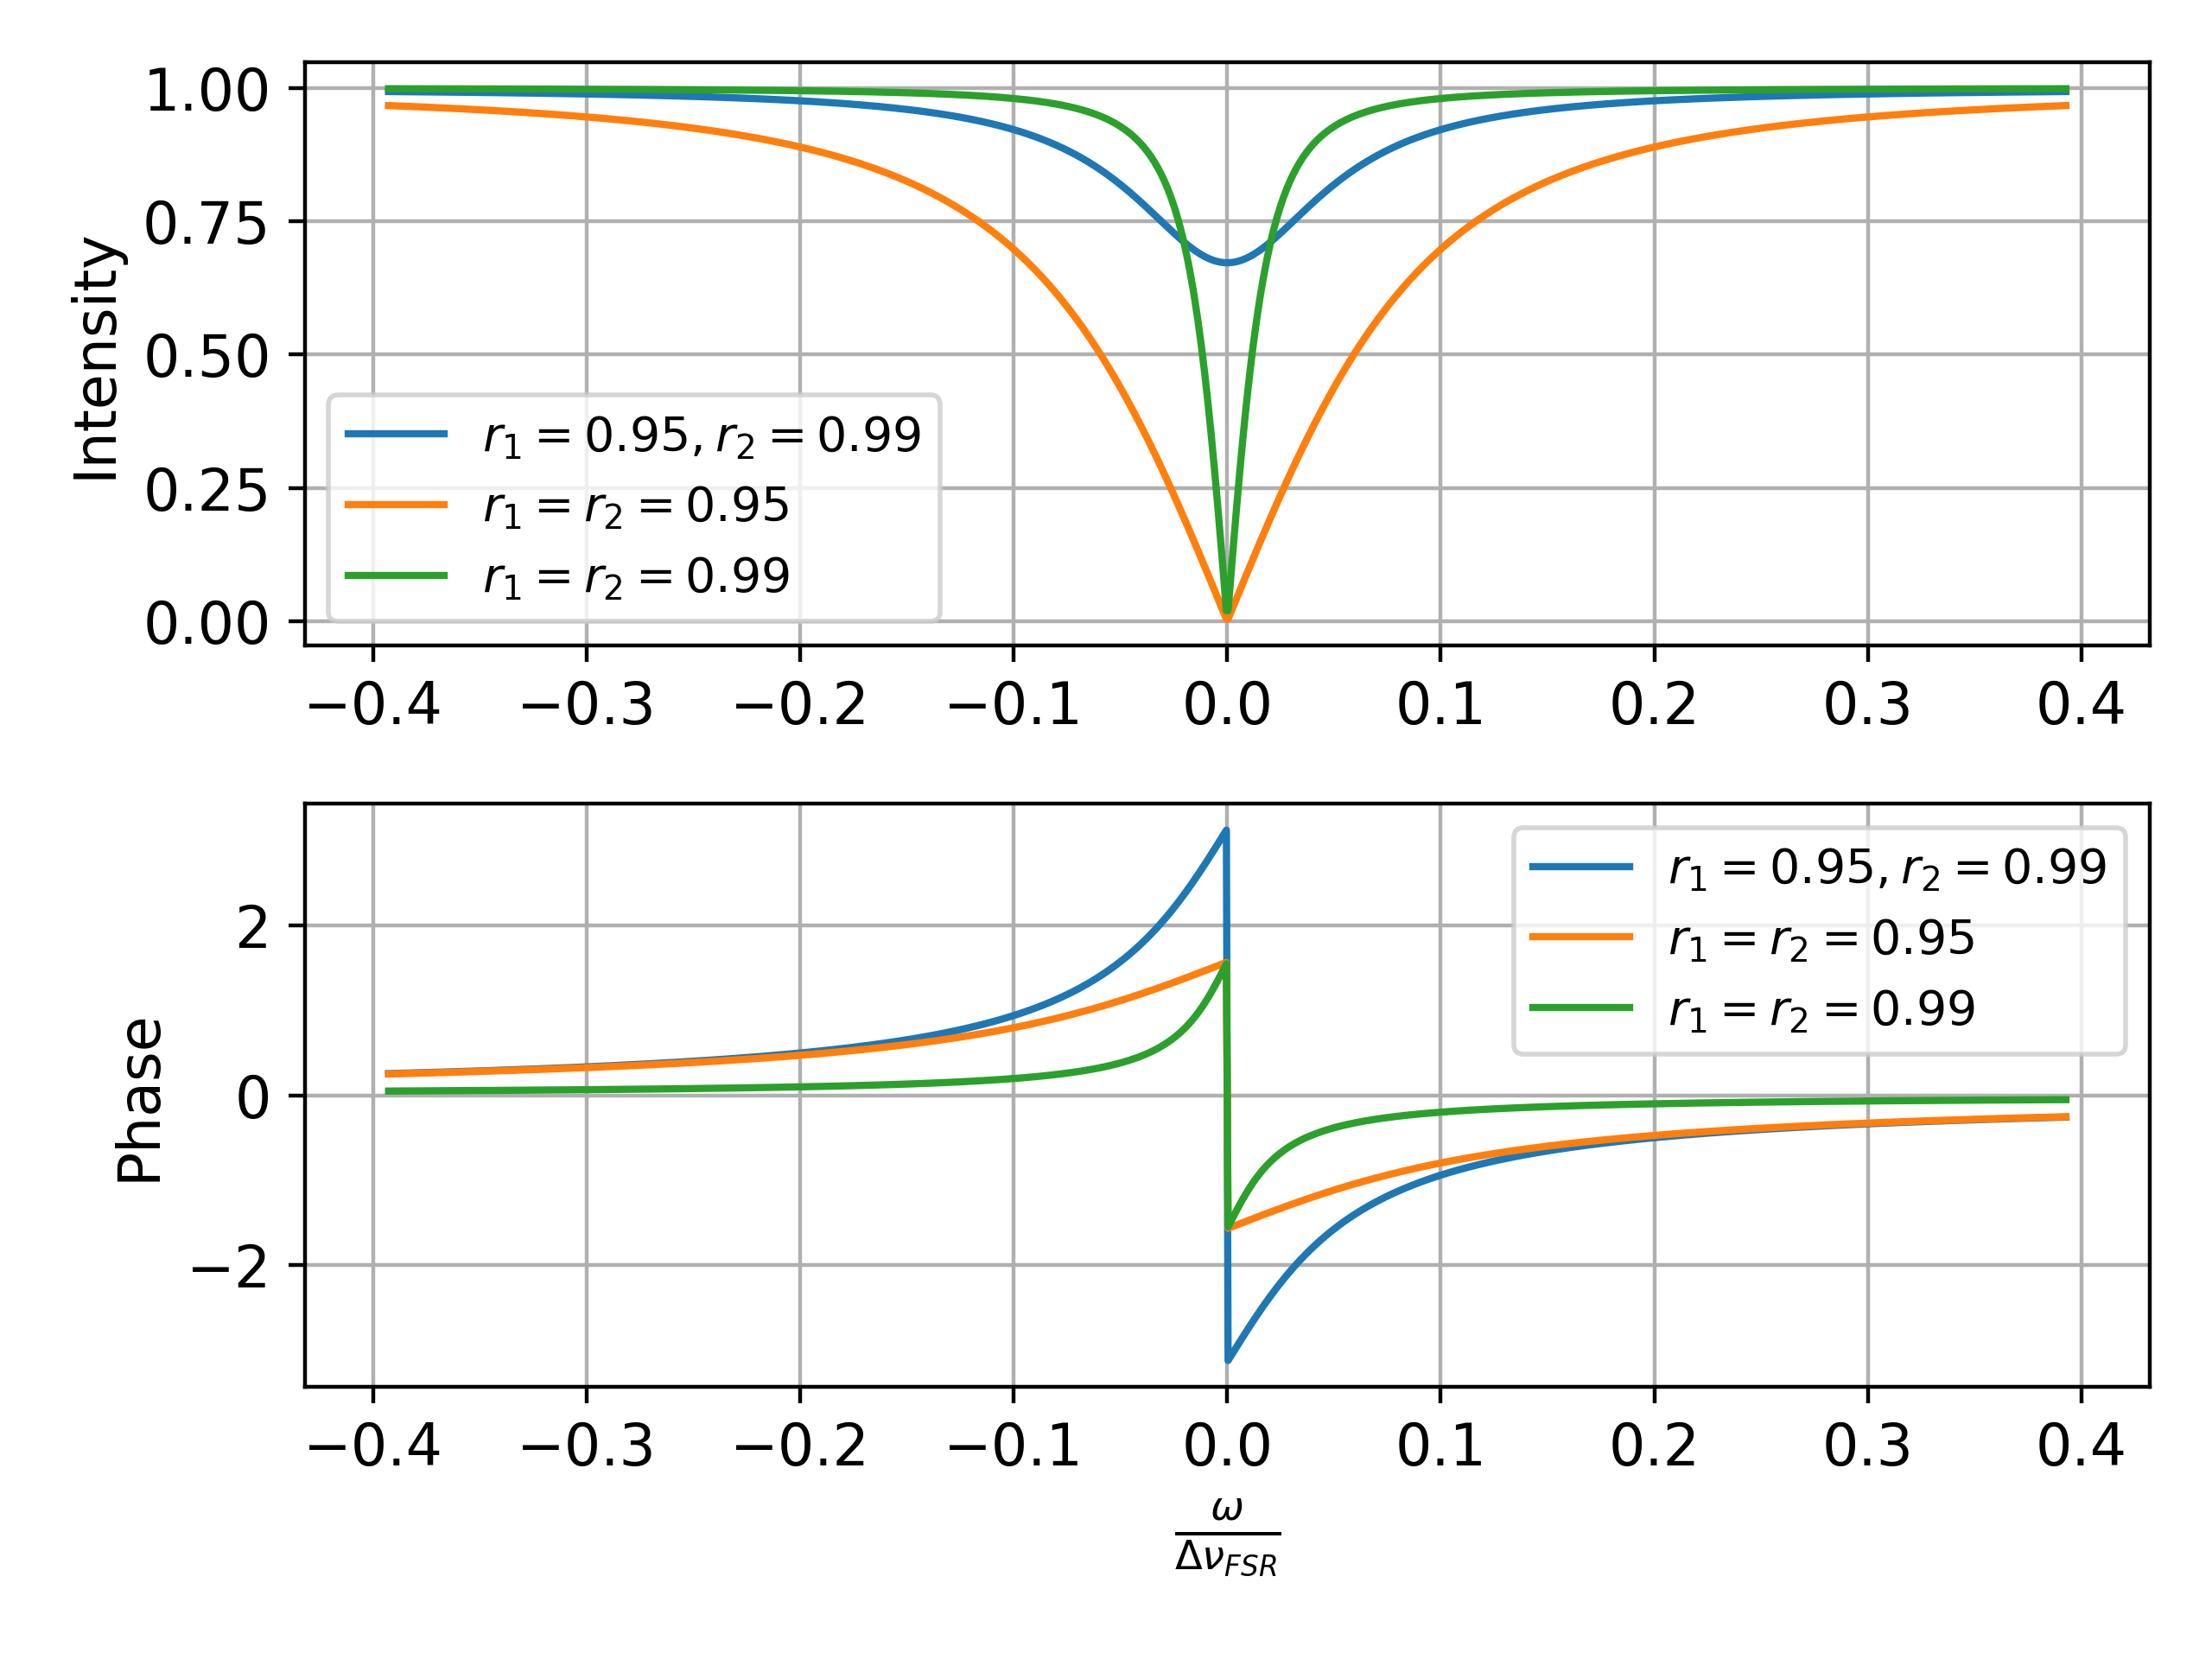
\includegraphics[width=\linewidth]{images/reflection_coefficient.png}
    \caption{Reflected light intensity and phase plot for different mirror reflection coefficients}
    \label{fig:reflection_coefficient}
\end{figure}
\section{PDH Locking}
PDH locking technique can be used to reduce the frequency noise of a laser using a stable reference cavity, or stabilise a cavity to a low-noise laser source. The simplified schematic in Fig. \ref{fig:pdh_schematic} shows the latter in which the cavity length is adjusted using a piezoelectric component. This configuration can compensate for any cavity drift (within reason) provided a stable laser. The same algorithm, in principle, can be applied to stabilising the laser frequency if we have actuators on the laser and a stable reference cavity. \par
\begin{figure}
    \centering
    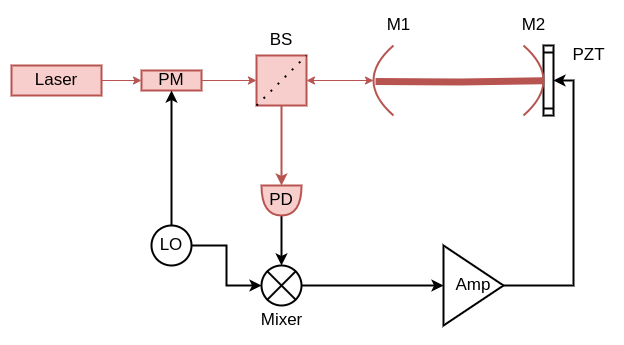
\includegraphics[width=\linewidth]{images/pdh_locking.drawio.png}
    \caption{Simplified schematic for PHD locking. A FP cavity is locked to a stable laser source. BS: Beam Splitter, PM : Phase Modulator. Red colour is the optical path, black colour is for electrical components/connections.}
    \label{fig:pdh_schematic}
\end{figure}
In the laser section, we saw that the reflected light changes its phase depending on which side of resonance it is on. However, the phase of the light, by itself, can't be measured by the electronic system we have at our disposal. PDH locking offers us a way to measure the phase of the reflected light indirectly by dithering the laser frequency. 
\subsection{Action of Phase Modulator}
We have been using phase modulators (PMs) extensively in our QKD chassis, and know that the electric field after passing through a PM is given by, 
\begin{equation}
    E_{\text{inc}}= E_0 e^{j(\omega t + \beta \sin \Omega t)}
\end{equation}
where $\omega$ is the frequency of light, and $\Omega$ is the modulation frequency. It can be expanded using Bessel function to \footnote{There is a useful identity involving Bessel functions given by $$
Ae^{j\omega t + j \beta \sin (\Omega t)} = A e^{j\omega t }(J_0(\beta)+\sum_k J_k (\beta)e^{jk\Omega t}+\sum_k (-1)^k J_k e^{-jk\Omega t}
$$
There are an infinite number of sidebands. The same can be achieved using Taylor expansion for the exponent and dropping the higher terms for our purpose. }
\begin{equation}
\label{eqn: pm_light}
    E_{\text{inc}} \approx [J_0 (\beta) + J_1(\beta) e^{j (\omega + \Omega)t} - J_1(\beta) e^{j (\omega - \Omega)t}]
\end{equation}
Eq. \ref{eqn: pm_light} shows that there are actually three frequencies incident on the cavity: a carrier, with frequency $\omega$ and two sidebands with frequencies $\omega \pm \Omega$. If the total incident power is given by $P_0 = |E_0|^2$, then the power in the carrier beam will be given by, 
\begin{equation}
    P_c = J_0^2(\beta) P_0
\end{equation}
and power in each first-order sideband is given by,  
\begin{equation}
    P_s = J_1^2(\beta) P_0
\end{equation}
If we keep the modulation depth small ($\beta  < 1$), almost all of the power will lie between the carrier and sidebands. An estimate of the modulation frequency $\Omega$ and modulation depth $\beta$ will be given in the simulation section.
\subsection{Modulated Beam on FP Cavity}
The reason for the elaborate explanation of resonant properties was to use the \textit{reflection coefficient} given by Eq. \ref{eqn: reflection coefficient} for each of the three beams independently. If the modulated beam is incident on the cavity, the reflected beam would be, 
\begin{equation}
\begin{split}
  E_{\text{refl}} =& E_0[F(\omega) J_0 (\beta) e^{j\omega t}+ F(\omega+ \Omega) J_1 (\beta) e^{j(\omega+\Omega) t}  \\
   &- F(\omega-\Omega) J_0 (\beta) e^{j(\omega - \Omega)t} ]
  \end{split}
\end{equation}
As photodiodes are intensity detectors, not field detectors, we will detect $P_{\text{refl}} = |E_{\text{refl}}|^2$. Simple algebra gives us, 
\begin{equation}
\label{eqn: reflected_power_modulated}
    \begin{split}
        P_{\text{refl}} = & |E_0|^2 \Big[|J_0|^2|F(\omega)|^2 + |J_1|^2\{|F(\omega+\Omega)|^2+|F(\omega-\Omega)|^2\} \\
        & + J_0 J_1 ^ *\{ F(\omega) F^*(\omega+\Omega)e^{-j\Omega t } - F(\omega) F^*(\omega-\Omega) e^{j\Omega t}\} \\
        & + J_0^* J_1\{ F^*(\omega) F(\omega+\Omega)e^{j\Omega t } - F^*(\omega) F(\omega-\Omega) e^{-j\Omega t}\} \Big] \\& +(2 \Omega \text{ terms } ) \\
        = &\Big[P_c|F(\omega)|^2 + P_s|\{F(\omega+\Omega)|^2+F(\omega-\Omega)|^2\} \\
        & + 2\sqrt{P_c P_s}\Big[ \mathrm{Re}\{F(\omega) F^*(\omega+\Omega) - F^*(\omega) F(\omega-\Omega)\}\cos \Omega t \\
        & \mathrm{Im}\{F(\omega) F^*(\omega+\Omega)- F^*(\omega) F(\omega-\Omega) \} \sin \Omega t \Big] +(2 \Omega \text{ terms } )\\
    \end{split}
\end{equation}
Eq. \ref{eqn: reflected_power_modulated} shows the interference of three waves. We will be interested in the frequency $\Omega$ which has two terms a sine and a cosine. This is achieved by using a high-bandwidth photodetector whose output is fed to the mixer with an LO signal. With the help of a low pass filter after that, we will be able to isolate our frequency of interest.
\subsection{Modulation Frequency}
There are two possible orders of modulating the phase modulator: one where the modulation frequency is slow. This means that the frequency of the cavity is varied slowly such that the standing waves inside the cavity are always in equilibrium with the incident beam. However, the beauty of PDH technique is that the error signal doesn't depend on the response time of the FB cavity itself. \par
If the cavity is near resonance and the modulation frequency is large enough, we can assume that the entire power in the sidebands is reflected, i.e. $F(\omega \pm \Omega) \approx 1$. The expression in Eq. \ref{eqn: reflected_power_modulated} would become, 
\begin{equation}
  F(\omega) F^*(\omega+\Omega) - F^*(\omega) F(\omega-\Omega) = 2 j~\mathrm{Im}\{F(\omega)\}
\end{equation}
This shows that at high modulation frequency, only Imaginary term of the two $\Omega$ is left from Eq. \ref{eqn: reflected_power_modulated}, and hence, our error signal becomes, 
\begin{equation}
    \epsilon \approx 2\sqrt{P_cP_s}~\mathrm{Im}\{F(\omega) F^*(\omega+\Omega)- F^*(\omega) F(\omega-\Omega) \}
\end{equation}
Fig. \ref{fig: pdh-error-signal} shows the plot of this error signal for fast modulation. The nature of the curve depends on the modulation depth, frequency $\Omega$ and the cavity among. We are still assuming the lossless case for our analysis. The error signal crosses zero every time the cavity is resonant with either the carrier or the sidebands. The opposite sign of the slope is useful if we accidentally lock to the sidebands. \par
\begin{figure}[h]
    \centering
    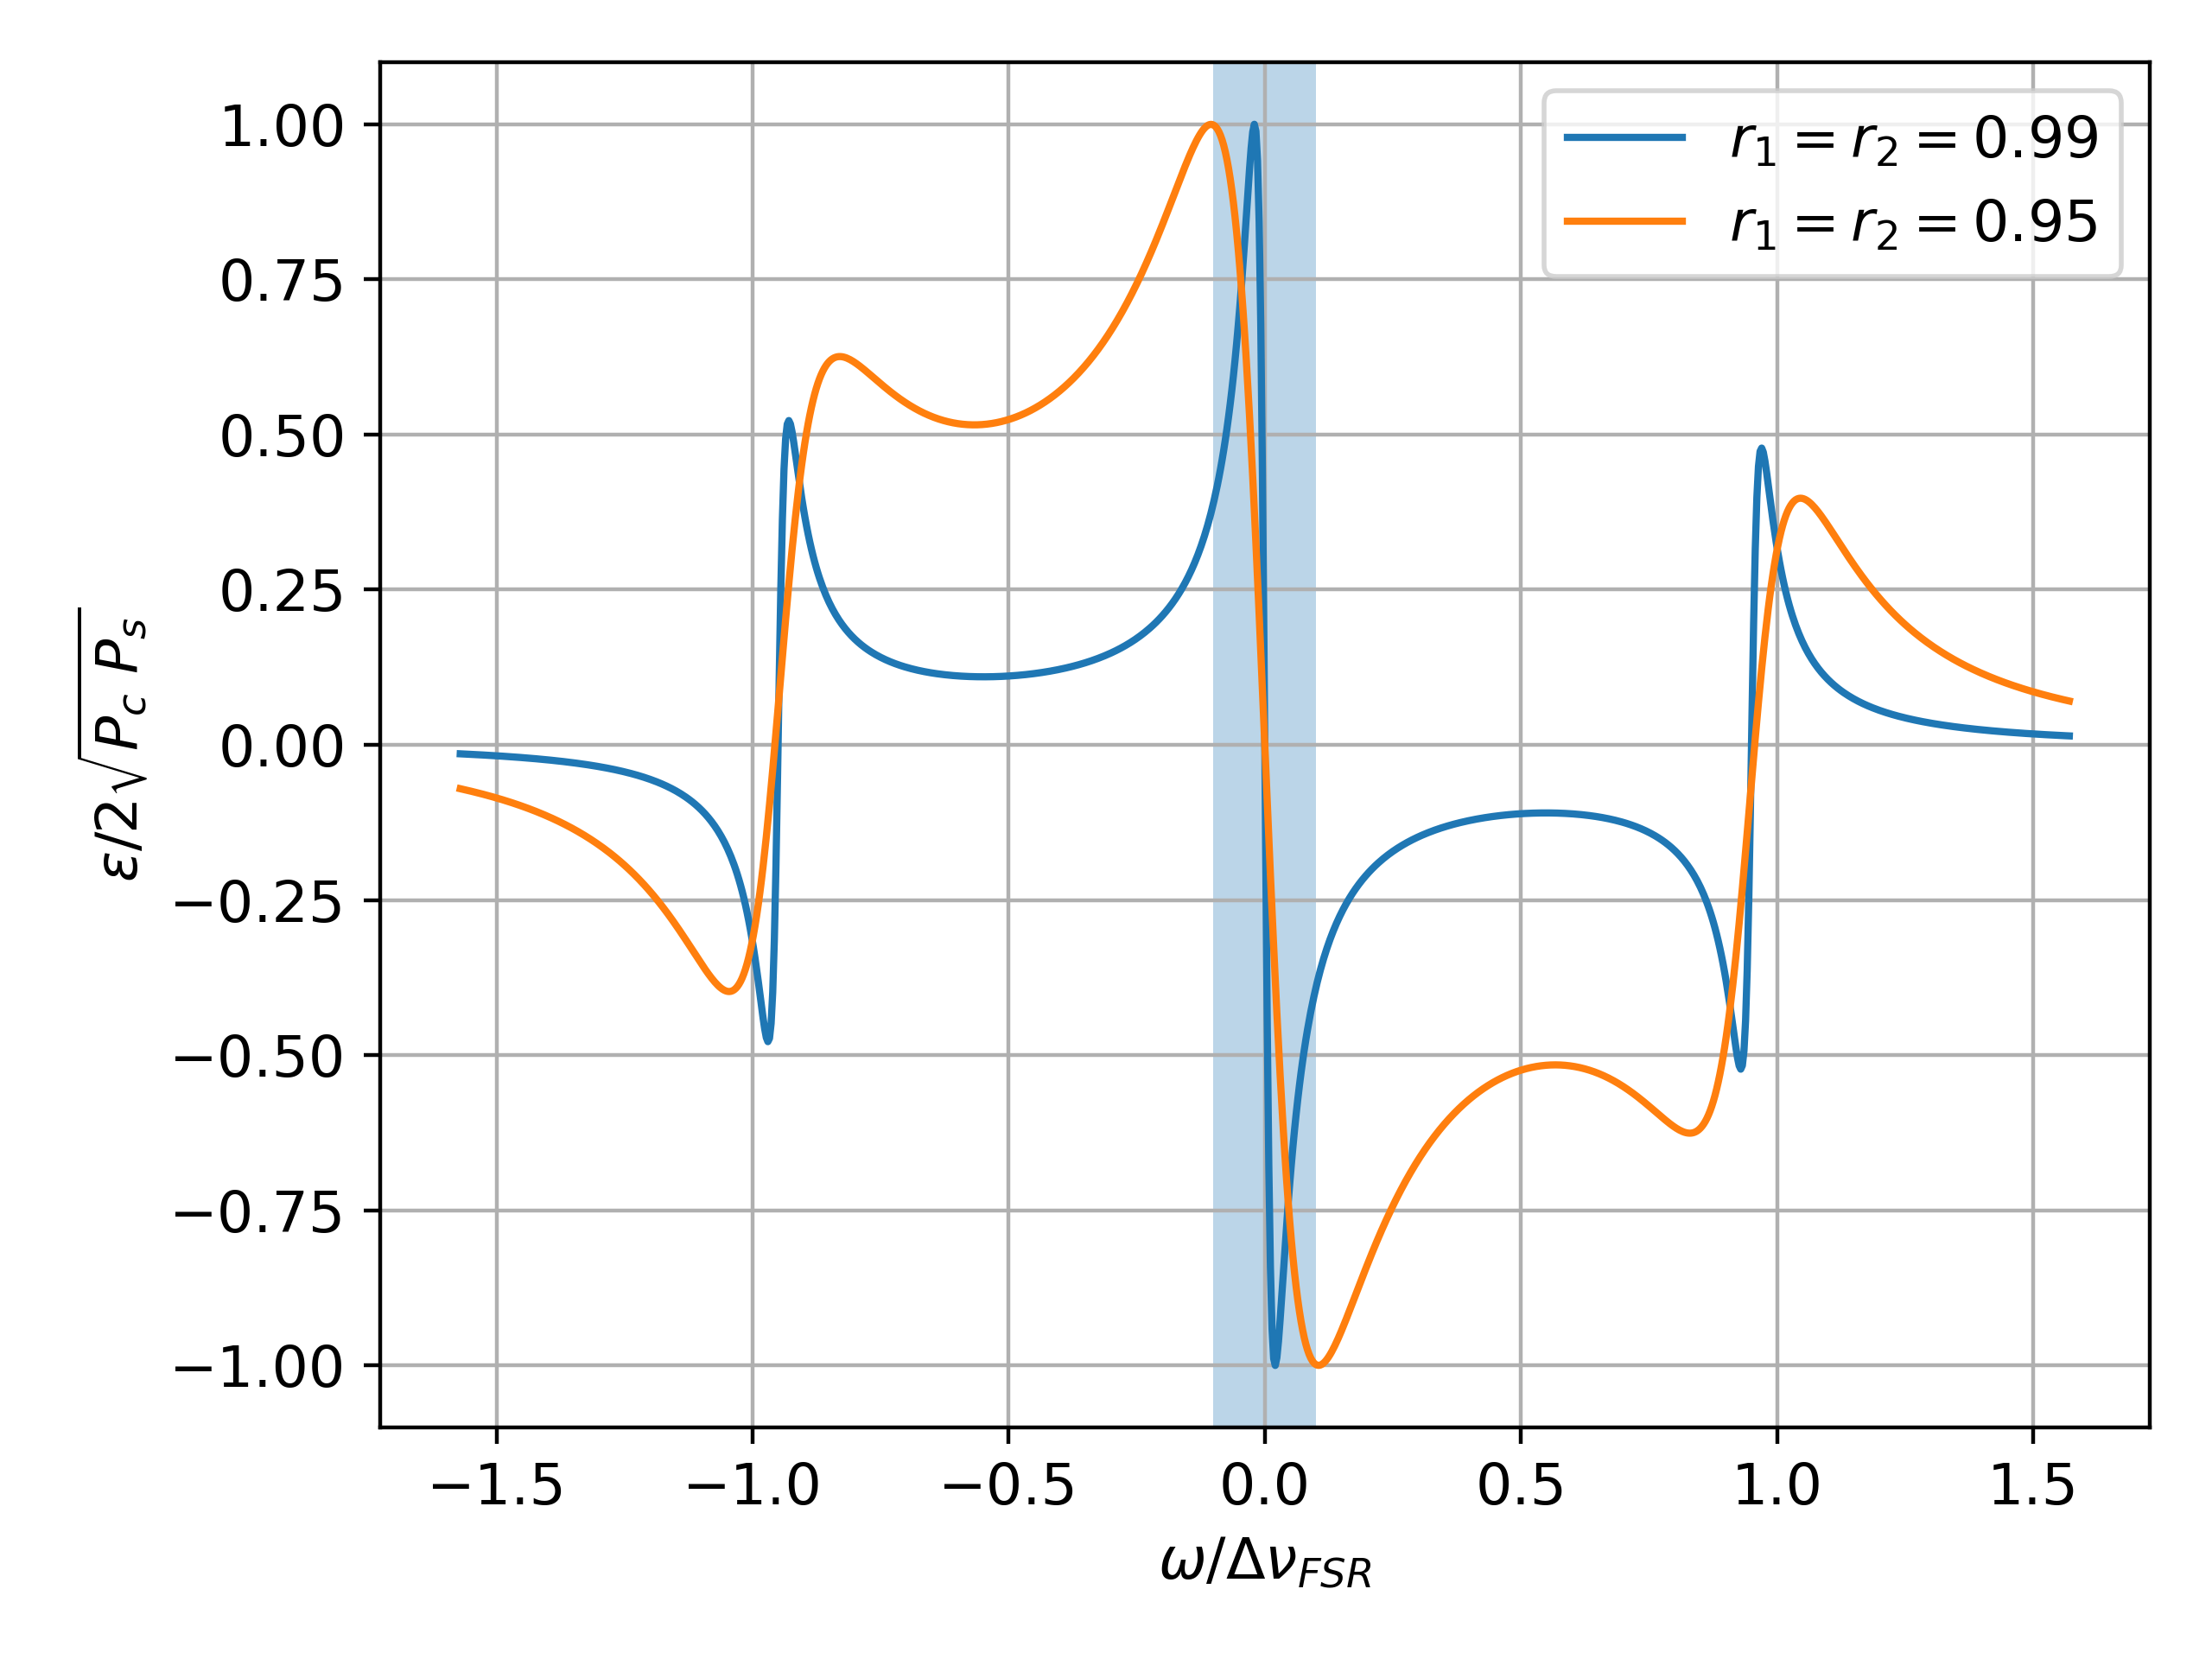
\includegraphics[width=\linewidth]{images/error_signal_depth_95.png}
    \caption{The error signal for fast modulation. The shape of the error signal changes with reflectivity of cavity.}
    \label{fig: pdh-error-signal}
\end{figure}
Near resonance, the reflected power essentially vanishes, since $|F \omega|^2 \approx 0$. The reflected power expression retains the first-order term given by to approximate the power, 
\begin{equation}
    P_{\text{refl}} \approx 2 P_s + 4 j~\mathrm{Im}\{F(\omega\}\sin \Omega t + (2\Omega ~\text{terms}~)
\end{equation}
Since the error signal is linear in offset from resonance, shown as the highlighted region in Fig. \ref{fig: pdh-error-signal}, we can use a PID controller with set point as zero. If it the system is locked to one of the sidebands, we will have to change the polarity of the control signal to compensate for the change in slope. 
\section{Building a cavity}
With the prerequisites described in the previous sections, we are ready to look at the available mirrors in the lab to build our cavity. The setup will be designed for 1064~nm. \par
\begin{table}[!h]
\centering
\begin{tabular}{|c|c|c|c|}
\hline
  Sl. &  Mirror & $r^2$ & ROC (mm) \\ \hline
    01 &PR1-1064-95-1025& $95\%$     & $\infty$ \\ \hline
    02 &PR1-1064-95-0.10CC & $95\%$ & 100 \\ \hline
    03 &E1705005MK2 (dual band - slightly broken ) & $99\%$ & 200\\
    \hline
\end{tabular}
    \caption{List of mirrors 1064~nm compatible mirrors available in the lab.}
    \label{tab: available_mirrors}
\end{table}
Using the mirrors available in Table \ref{tab: available_mirrors}, I would look at different cavity configurations. The parameter, primarily considered, is the cavity linewidth, as it decides the modulation frequency ($\Omega \gg\text{FWHM}$). 
\subsection{Cavity Parameters}
\lipsum[2]\cite{latex:companion}. \par
\section{Remarks}
\lipsum[4]
\bibliography{sample}
\end{document}
